\let\negmedspace\undefined
\let\negthickspace\undefined
\documentclass[journal]{IEEEtran}
\usepackage[a5paper, margin=10mm, onecolumn]{geometry}
%\usepackage{lmodern} % Ensure lmodern is loaded for pdflatex
\usepackage{tfrupee} % Include tfrupee package

\setlength{\headheight}{1cm} % Set the height of the header box
\setlength{\headsep}{0mm}     % Set the distance between the header box and the top of the text

\usepackage{gvv-book}
\usepackage{gvv}
\usepackage{cite}
\usepackage{amsmath,amssymb,amsfonts,amsthm}
\usepackage{algorithmic}
\usepackage{graphicx}
\usepackage{textcomp}
\usepackage{xcolor}
\usepackage{txfonts}
\usepackage{listings}
\usepackage{enumitem}
\usepackage{mathtools}
\usepackage{gensymb}
\usepackage{comment}
\usepackage[breaklinks=true]{hyperref}
\usepackage{tkz-euclide}
\usepackage{multicol}
\usepackage{listings}
                                        
\def\inputGnumericTable{}                                 
\usepackage[latin1]{inputenc}                                
\usepackage{color}                                            
\usepackage{array}                                            
\usepackage{longtable}                                       
\usepackage{calc}                                             
\usepackage{multirow}                                         
\usepackage{hhline}
\usepackage{ifthen}                                           
\usepackage{lscape}
\usepackage{circuitikz}


\renewcommand{\thefigure}{\theenumi}
\renewcommand{\thetable}{\theenumi}
\setlength{\intextsep}{10pt} % Space between text and floats


\numberwithin{equation}{enumi}
\numberwithin{figure}{enumi}
\renewcommand{\thetable}{\theenumi}


% Marks the beginning of the document
\begin{document}
\bibliographystyle{IEEEtran}



\begin{center}
    \LARGE \textbf{GATE 2015 MA}\\[0.5em]
    \large \textbf{AI25BTECH11012 - UNNATHI GARIGE}
\end{center}

 \textbf{Q.1-Q.5 carry one mark each.}

 \begin{enumerate}
     \item Choose the appropriate word/phrase, out of the four options given below, to complete the following sentence:\\
Apparent lifelessness \underline{\hspace{2cm}} dormant life.
\hfill{\text{GATE MA 2015}}
\begin{multicols}{4}
\begin{enumerate}
    \item harbours
    \item leads to
    \item supports
    \item affects
\end{enumerate}
\end{multicols}


\item Fill in the blank with the correct idiom/phrase. \hfill{\text{GATE MA 2015}}
That boy from the town was a \underline{\hspace{2cm}} in the sleepy village.
\hfill{\text{GATE MA 2015}}
\begin{multicols}{2}
\begin{enumerate}
    \item dog out of herd
    \item sheep from the heap
    \item fish out of water
    \item bird from the flock
\end{enumerate}
\end{multicols}


\item Choose the statement where underlined word is used correctly.
\hfill{\text{GATE MA 2015}}
\begin{enumerate}
    \item When the teacher eludes to different authors, he is being \underline{elusive}.
    \item When the thief keeps eluding the police, he is being \underline{elusive}.
    \item Matters that are difficult to understand, identify or remember are \underline{allusive}.
    \item Mirages can be \underline{allusive}, but a better way to express them is illusory.
\end{enumerate}


\item Tanya is older than Eric.
Cliff is older than Tanya. 
Eric is older than Cliff. 

If the first two statements are true, then the third statement is:
\hfill{\text{GATE MA 2015}}
\begin{enumerate}
    \item True
    \item False
    \item Uncertain
    \item Data insufficient
\end{enumerate}

\item Five teams have to compete in a league, with every team playing every other team exactly once, before going to the next round. How many matches will have to be held to complete the league round of matches?
\hfill{\text{GATE MA 2015}}
\begin{multicols}{4}
\begin{enumerate}
    \item 20
    \item 10
    \item 8
    \item 5
\end{enumerate}
\end{multicols}


\textbf{Q.6-Q.10 carry two mark each.}
\bigskip
\item Select the appropriate option in place of underlined part of the sentence.

\underline{Increased productivity necessary} reflects greater efforts made by the employees.

\begin{enumerate}
    \item Increase in productivity necessary \hfill{\text{GATE MA 2015}}
    \item Increase productivity is necessary
    \item Increase in productivity necessarily
    \item No improvement required
\end{enumerate}

\item Given below are two statements followed by two conclusions. Assuming these statements to be true, decide which one logically follows. \hfill{\text{GATE MA 2015}}

Statements:
\begin{enumerate}
    \item[I.] No manager is a leader.
    \item[II.] All leaders are executives.
\end{enumerate}

Conclusions:
\begin{enumerate}
    \item[I.] No manager is an executive.
    \item[II.] No executive is a manager.
\end{enumerate}
\begin{enumerate}
    \item Only conclusion I follows.
    \item Only conclusion II follows.
    \item Neither conclusion I nor II follows.
    \item Both conclusions I and II follow.
\end{enumerate}

\item In the given figure angle $Q$ is a right angle. $PS:QS=3:1$, $RT:QT=5:2$ and $PU:UR=1:1$. If area of triangle $QTS$ is $20\,\mathrm{cm}^2$, then the area of triangle $PQR$ in $\mathrm{cm}^2$ is \underline{\hspace{2cm}}. 
\hfill{\text{GATE MA 2015}}
\vspace{1em}

\begin{figure}[ht!]
    \centering
    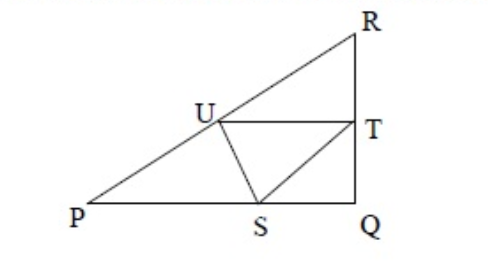
\includegraphics[width=0.35\textwidth]{ques_8.png}
    \caption{}
    \label{fig:fig1.jpeg}
\end{figure}

\item constructed in the $xy$-plane so that the right angle is at $P$ and line $PR$ is parallel to the $x$-axis. The $x$ and $y$ coordinates of $P$, $Q$, and $R$ are to be integers that satisfy the inequalities: $-4 \leq x \leq 5$ and $6 \leq y \leq 16$. How many different triangles could be constructed with these properties?
\hfill{\text{GATE MA 2015}}
\begin{multicols}{4}
\begin{enumerate}
    \item 110
    \item 1100
    \item 9900
    \item 10000
\end{enumerate}
\end{multicols}


\item A coin is tossed thrice. Let $X$ be the event that head occurs in each of the first two tosses. Let $Y$ be the event that a tail occurs on the third toss. Let $Z$ be the event that two tails occur in three tosses. Based on the above information, which one of the following statements is TRUE?
\hfill{\text{GATE MA 2015}}
\begin{multicols}{2}
\begin{enumerate}
    \item $X$ and $Y$ are not independent
    \item $Y$ and $Z$ are dependent
    \item $Y$ and $Z$ are independent
    \item $X$ and $Z$ are independent
\end{enumerate}
\end{multicols}

\textbf{Q.11 to Q.35 carry one mark each.}


\item Let $T: \mathbb{R}^4 \to \mathbb{R}^4$ be a linear map defined by  \hfill{\text{GATE MA 2015}}
\begin{align*}
T(x, y, z, w) = (x + z,\ 2x + y + 3z,\ 2y + 2z, w).
\end{align*}
Then the rank of $T$ is equal to \underline{\hspace{2cm}}.
\vspace{1em}

\item Let $M$ be a $3 \times 3$ matrix and suppose that $1, 2$ and $3$ are the eigenvalues of $M$. \\
If  \hfill{\text{GATE MA 2015}}
\begin{align*}
M^{-1} = \frac{M^2 - M + I_3}{\alpha}
\end{align*}
for some scalar $\alpha \neq 0$, then $\alpha$ is equal to \underline{\hspace{2cm}}.
\vspace{1em}

\item Let $M$ be a $3 \times 3$ singular matrix and suppose that $2$ and $3$ are eigenvalues of $M$. Then the number of linearly independent eigenvectors of $M^3 + 2M + I_3$ is equal to \underline{\hspace{2cm}}. \hfill{\text{GATE MA 2015}}
\vspace{1em}

\item Let $M$ be a $3 \times 3$ matrix such that $M \myvec{ -2 \\ 1 \\ 0 } = \myvec{ 6 \\ -3 \\ 0 }$ and suppose that $M^3 \myvec{ 1 \\ -1/2 \\ 0 } = \myvec{ \alpha \\ \beta \\ \gamma }$ for some $\alpha, \beta, \gamma \in \mathbb{R}$. Then $|\alpha|$ is equal to \underline{\hspace{2cm}}.
\hfill{\text{GATE MA 2015}}
\vspace{1em}

\item Let \( f: [0, \infty) \to \mathbb{R} \) be defined by
\begin{align*}
f(x) = \int_0^x \sin^2(t^2)\,dt.
\end{align*}
Then the function \( f \) is:  \hfill{\text{GATE MA 2015}}
\begin{enumerate}
    \item uniformly continuous on \([0, 1]\) but NOT on \((0, \infty)\)
    \item uniformly continuous on \((0, \infty)\) but NOT on \([0, 1]\)
    \item uniformly continuous on both \([0, 1]\) and \((0, \infty)\)
    \item neither uniformly continuous on \([0,1]\) nor uniformly continuous on \((0, \infty)\)
\end{enumerate}


\item Consider the power series \( \sum_{n=0}^{\infty} a_n z^n \), where
\hfill{\text{GATE MA 2015}}
\begin{align*}
a_n = \begin{cases}
    \frac{1}{3^n} & \text{if $n$ is even} \\
    \frac{1}{5^n} & \text{if $n$ is odd}
\end{cases}
\end{align*}
The radius of convergence of the series is equal to \underline{\hspace{2cm}}.
\vspace{1em}


\item Let \( C = \{ z \in \mathbb{C} : |z - i| = 2 \} \). Then
\hfill{\text{GATE MA 2015}}
\begin{align*}
\frac{1}{2\pi i} \oint_C \frac{z^2 - 4}{z^2 + 4}\,dz
\end{align*}
is equal to  \underline{\hspace{2cm}}.
\vspace{1em}

\item Let \( X \sim B\left(5, \frac{1}{2}\right) \) and \( Y \sim U(0,1) \).
Then 
\hfill{\text{GATE MA 2015}}
\begin{align*}
\frac{P(X + Y \leq 2)}{P(X + Y \geq 5)}
\end{align*}
is equal to \underline{\hspace{2cm}}.
\vspace{1em}

\item Let the random variable \( X \) have the distribution function
\hfill{\text{GATE MA 2015}}
\begin{align*}
F(x) = 
\begin{cases}
0 & \text{if } x < 0 \\[8pt]
\frac{x}{2} & \text{if } 0 \leq x < 1 \\[8pt]
\frac{3}{5} & \text{if } 1 \leq x < 2 \\[8pt]
\frac{1}{2} + \frac{x}{8} & \text{if } 2 \leq x < 3 \\[8pt]
1 & \text{if } x \geq 3
\end{cases}
\end{align*}
Then \( P(2 \leq X < 4) \) is equal to \underline{\hspace{2cm}}.

\item Let \( X \) be a random variable having the distribution function
\hfill{\text{GATE MA 2015}}
\begin{align*}
F(x) = 
\begin{cases}
0 & \text{if } x < 0 \\[8pt]
\frac{1}{4} & \text{if } 0 \leq x < 1 \\[8pt]
\frac{1}{3} & \text{if } 1 \leq x < 2 \\[8pt]
\frac{1}{2} & \text{if } 2 \leq x < \frac{11}{3} \\[8pt]
1 & \text{if } x \geq \frac{11}{3}
\end{cases}
\end{align*}
Then \( E(X) \) is equal to \underline{\hspace{2cm}}.


\item In an experiment, a fair die is rolled until two sixes are obtained in succession. The probability that the experiment will end in the fifth trial is equal to
\hfill{\text{GATE MA 2015}}
\begin{multicols}{4}
\begin{enumerate}
    \item \( \dfrac{125}{6^5} \)
    \item \( \dfrac{150}{6^5} \)
    \item \( \dfrac{175}{6^5} \)  
    \item \( \dfrac{200}{6^5} \)
\end{enumerate}
\end{multicols}


\item Let \( x_1 = 2.2, \ x_2 = 4.3, \ x_3 = 3.1, \ x_4 = 4.5, \ x_5 = 1.1, \ x_6 = 5.7 \) be the observed values of a random sample of size 6 from a \( U(0-\theta, 0+\theta) \) distribution, where \( \theta \in (0, \infty) \) is unknown. Then a maximum likelihood estimate of \( \theta \) is equal to\\

.  \hfill{\text{GATE MA 2015}}
\begin{multicols}{4}
\begin{enumerate}
    \item 1.8
    \item 2.3
    \item 3.1 
    \item 3.6
\end{enumerate}
\end{multicols}



\item Let $\Omega = \{ (x, y) \in \mathbb{R}^2 \mid x^2 + y^2 < 1 \}$ be the open unit disc in $\mathbb{R}^2$ with boundary $\partial\Omega$. If $u(x, y)$ is the solution of the Dirichlet problem
\begin{align*}
\begin{cases}
u_{xx} + u_{yy} = 0 & \text{in } \Omega \\
u(x,y) = 1 - 2y^2 & \text{on } \partial\Omega
\end{cases}
\end{align*}
then $u\left( \frac{1}{2}, 0 \right)$ is equal to
 \hfill{\text{GATE MA 2015}}
\begin{multicols}{4}
\begin{enumerate}
    \item -1
    \item $-\frac{1}{4}$ 
    \item $\frac{1}{4} $
    \item 1
\end{enumerate}
\end{multicols}


\item Let $c \in \mathbb{Z}$ be such that 
\begin{align*}
\frac{\mathbb{Z}(x)}{x^2 + x + c}
\end{align*} is a field. Then $c$ is equal to \underline{\hspace{2cm}}.
 \hfill{\text{GATE MA 2015}}
\vspace{1em}

\item Let $V = C^1[0, 1]$, $X = (C[0, 1], \ \| \cdot \|{\infty})$ and $Y = (C[0, 1], \ \| \cdot \|{2})$. \\
Then $V$ is
 \hfill{\text{GATE MA 2015}}
\begin{enumerate}
\item  dense in $X$ but NOT in $Y$
\item dense in $Y$ but NOT in $X$
\item dense in both $X$ and $Y$
\item neither dense in $X$ nor dense in $Y$
\end{enumerate}

\item Let $T : (C[0, 1], \|\cdot\|{\infty}) \to \mathbb{R}$ be defined by $T(f) = \int_0^1 2x f(x) \, dx$ for all $f \in C[0, 1]$. Then $\|T\|$ is equal to \underline{\hspace{2cm}}.
 \hfill{\text{GATE MA 2015}}
\vspace{1em}

\item Let $\tau_1$ be the usual topology on $\mathbb{R}$. Let $\tau_2$ be the topology on $\mathbb{R}$ generated by 
\begin{align*}
\mathcal{B} = \{ [a,b) \subset \mathbb{R} : -\infty < a < b < \infty \}.
\end{align*} 

Then the set $\left\{ x \in \mathbb{R} : 4 \sin^2 x \leq 1 \right\} \cup \left\{ \frac{\pi}{2} \right\}$ is
\hfill{\text{GATE MA 2015}}
\begin{enumerate}
 \item  closed in $(\mathbb{R}, \tau_1)$ but NOT in $(\mathbb{R}, \tau_2)$
 \item  closed in $(\mathbb{R}, \tau_2)$ but NOT in $(\mathbb{R}, \tau_1)$
 \item  closed in both $(\mathbb{R}, \tau_1)$ and $(\mathbb{R}, \tau_2)$
 \item  neither closed in $(\mathbb{R}, \tau_1)$ nor closed in $(\mathbb{R}, \tau_2)$
\end{enumerate}

\item Let $X$ be a connected topological space such that there exists a non-constant continuous function $f : X \to \mathbb{R}$, where $\mathbb{R}$ is equipped with the usual topology. Let $f(X) = \{ f(x) : x \in X \}$. Then
\hfill{\text{GATE MA 2015}}
\begin{enumerate}
 \item  $X$ is countable but $f(X)$ is uncountable
 \item  closed in $(\mathbb{R}, \tau_2)$ but NOT in $(\mathbb{R}, \tau_1)$
 \item  both $f(X)$ and $X$ are countable
 \item both $f(X)$ and $X$ are uncountable
\end{enumerate}


\item Let $d_1$ and $d_2$ denote the usual metric and the discrete metric on $\mathbb{R}$, respectively. Let $f : (\mathbb{R}, d_1) \to (\mathbb{R}, d_2)$ be defined by $f(x) = x$, $x \in \mathbb{R}$. Then \hfill{\text{GATE MA 2015}}
\begin{enumerate}
\item  $f$ is continuous but $f^{-1}$ is NOT continuous
\item  $f^{-1}$ is continuous but $f$ is NOT continuous
\item  both $f$ and $f^{-1}$ are continuous
\item  neither $f$ nor $f^{-1}$ is continuous
\end{enumerate}


\item If the trapezoidal rule with single interval $[0,1]$ is exact for approximating the integral

\begin{align*}
\int_{0}^{1} (x^3 - c x^2) \, dx,
\end{align*}
then the value of $c$ is equal to \underline{\hspace{2cm}}.   \hfill{\text{GATE MA 2015}}
\vspace{1em}

\item Suppose that the Newton-Raphson method is applied to the equation $2x^2 + 1 - e^{x^2} = 0$ with an initial approximation $x_0$ sufficiently close to zero. Then, for the root $x = 0$, the order of convergence of the method is equal to \underline{\hspace{2cm}}\\ .  \hfill{\text{GATE MA 2015}}

\item The minimum possible order of a homogeneous linear ordinary differential equation with real constant coefficients having $x^2 \sin(x)$ as a solution is equal to \underline{\hspace{2cm}} \\
. \hfill{\text{GATE MA 2015}}
\vspace{1em}

\item The Lagrangian of a system in terms of polar coordinates $(r, \theta)$ is given by
\begin{align*}
L = \frac{1}{2} m r^2 + \frac{1}{2} m ( r^2 + r^2 \dot{\theta}^2 ) - m g r ( 1 - \cos(\theta) ),
\end{align*}
where $m$ is the mass, $g$ is the acceleration due to gravity and $\dot{s}$ denotes the derivative of $s$ with respect to time. Then the equations of motion are
\hfill{\text{GATE MA 2015}}
\begin{enumerate}
\item  $ 2 \ddot{r} = r \dot{\theta}^2 - g\, (1 - \cos(\theta)), \frac{d}{dt}(r^2 \dot{\theta}) = -g\, r\, \sin(\theta)$ 
\item   $2 \ddot{r} = r \dot{\theta}^2 + g\, (1 - \cos(\theta)),  \frac{d}{dt}(r^2 \dot{\theta}) = -g\, r\, \sin(\theta)$ 
\item   $\ddot{r} = r \dot{\theta}^2 - g\, (1 - \cos(\theta)),  \frac{d}{dt}(r^2 \dot{\theta}) = g\, r\, \sin(\theta)$ 
\item  $\ddot{r} = r \dot{\theta}^2 + g\, (1 - \cos(\theta)),  \frac{d}{dt}(r^2 \dot{\theta}) = g\, r\, \sin(\theta)$
\end{enumerate}


\item If $y(x)$ satisfies the initial value problem  \hfill{\text{GATE MA 2015}}
\begin{align*}
(x^2 + y) dx = x\, dy, \qquad y(1) = 2,
\end{align*}
then $y(2)$ is equal to \underline{\hspace{2cm}}
\vspace{1em}

\item It is known that Bessel functions $I_n(x)$, for $n \geq 0$, satisfy the identity
\begin{align*}
e^{\frac{x}{2} (t - \frac{1}{t})} = J_0(x) + \sum_{n=1}^{\infty} J_n(x) \left( t^n + \frac{(-1)^n}{t^n} \right)
\end{align*}
for all $t > 0$ and $x \in \mathbb{R}$. The value of $J_0\left(\frac{\pi}{2}\right) + 2 \sum_{n=1}^{\infty} J_{2n}\left(\frac{\pi}{2}\right)$ is equal to \underline{\hspace{2cm}}\\
 . \hfill{\text{GATE MA 2015}}

 \textbf{Q.36 to Q.65 carry two marks each.}

\item Let $X$ and $Y$ be two random variables having the joint probability density function
\begin{align*}
f(x, y) = 
\begin{cases}
2 & \text{if } 0 < x < y < 1 \\
0 & \text{otherwise}
\end{cases}
\end{align*}
Then the conditional probability $P \left( X \leq \frac{2}{3} \ \middle| \ Y = \frac{3}{4} \right)$ is equal to
 \hfill{\text{GATE MA 2015}}
 \begin{multicols}{4}
\begin{enumerate}
\item  $\frac{5}{9}$ 
\item  $\frac{2}{3}$
\item  $\frac{7}{9}$ 
\item  $\frac{8}{9}$
\end{enumerate}
\end{multicols}

\item Let $\Omega = [0, 1]$ be the sample space and let $P(\cdot)$ be a probability function defined by
\begin{align*}
P((0, x]) = 
\begin{cases}
\frac{1}{2} & \quad \text{if } 0 \leq x \leq \frac{1}{2} \\
x & \quad \text{if } \frac{1}{2} < x \leq 1
\end{cases}
\end{align*}
Then $P\left( \left(0, \frac{1}{2}\right] \right)$ is equal to \underline{\hspace{2cm}}
 \hfill{\text{GATE MA 2015}}
\vspace{1em}


 \item Let $X_1, X_2, X_3$ be independent and identically distributed random variables with $E(X_1) = 0$ and $E(X_1^2) = \frac{15}{4}$. If $\psi : (0, \infty) \to (0, \infty)$ is defined through the conditional expectation
\begin{align*}
\psi(t) = E(X_1^2 \mid X_1^2 + X_2^2 + X_3^2 = t), \quad t > 0,
\end{align*}
then $E\left(\psi((X_1^2 + X_2^2))\right)$ is equal to \underline{\hspace{2cm}}
 \hfill{\text{GATE MA 2015}} 
 \vspace{1em}

 \item Let $X \sim \mathrm{Poisson}(\lambda)$, where $\lambda > 0$ is unknown. If $f(X)$ is the unbiased estimator of $g(\lambda) = e^{-\lambda}(3\lambda^2 + 2\lambda + 1)$, then $\sum_{k=0}^\infty \delta(k)$ is equal to  \underline{\hspace{2cm}}\\
 . \hfill{\text{GATE MA 2015}}

\item Let $x_1, \ldots, x_n$ be a random sample from $N(\mu, 1)$ distribution, where $\mu \in \{0, \frac{1}{2}\}$. For testing the null hypothesis $H_0: \mu = 0$ against the alternative hypothesis $H_1: \mu = \frac{1}{2}$, consider the critical region
\begin{align*}
R = \left\{ (x_1, x_2, \ldots, x_n) : \sum_{i=1}^n x_i > c \right\}
\end{align*}
where $c$ is some real constant. If the critical region $R$ has size $0.025$ and power $0.7054$, then the value of the sample size $n$ is equal to \underline{\hspace{2cm}}\\
. \hfill{\text{GATE MA 2015}}


\item Let $X$ and $Y$ be independently distributed central chi-squared random variables with degrees of freedom $m$ ($\geq 3$) and $n$ ($\geq 3$) respectively. If $E\left(\frac{X}{X+Y}\right) = \frac{3}{7}$ and $m + n = 14$, then $E\left(\frac{Y}{X+Y}\right)$ is equal to
\hfill{\text{GATE MA 2015}}
\begin{multicols}{4}
\begin{enumerate}
 \item  $\frac{2}{7}$ 
 \item  $\frac{3}{14}$ 
 \item  $\frac{4}{7}$ 
 \item  $\frac{5}{7}$
\end{enumerate}
\end{multicols}


\item Let $X_1, X_2, \ldots$ be a sequence of independent and identically distributed random variables with
\begin{align*}
P(X_1 = 1) = \frac{1}{4} \quad \text{and} \quad P(X_1 = 2) = \frac{3}{4}.
\end{align*}
If $X_n = \frac{1}{n} \sum_{i=1}^{n} X_i$, for $n = 1, 2, \ldots$, then
$\lim_{n \to \infty} P(X_n \leq 1.8) \text{ is equal to }$ \underline{\hspace{2cm}}
\hfill{\text{GATE MA 2015}}

\item 
Let $u(x, y) = 2f(y)\cos(x - 2y)$, $(x, y) \in \mathbb{R}^2$, be a solution of the initial value problem
\begin{align*}
2u_x + u_y = u,\\
u(x, 0) = \cos(x).
\end{align*}
Then $f(1)$ is equal to
\hfill{\text{GATE MA 2015}}
\begin{multicols}{4}
\begin{enumerate}
   
    \item $\frac{1}{2}$
    \item $\frac{i}{2}$
    \item $e$
    \item $\frac{3e}{2}$
 
\end{enumerate}
\end{multicols}

\item Let $u(x, t),~x \in \mathbb{R},~t \geq 0$, be the solution of the initial value problem 
\begin{align*}
u_{tt} = u_{xx} \\
u(x, 0) = x\\
u_t(x, 0) = 1
\end{align*}

Then $u(2,2)$ is equal to \underline{\hspace{2cm}}
\hfill{\text{GATE MA 2015}}

\item Let $W = \operatorname{Span} \left\{ \frac{1}{\sqrt{2}} (0,0,1,1), \frac{1}{\sqrt{2}} (1,-1,0,0) \right\}$ be a subspace of the Euclidean space $\mathbb{R}^4$. Then the square of the distance from the point $(1,1,1,1)$ to the subspace $W$ is equal to \underline{\hspace{2cm}}
\hfill{\text{GATE MA 2015}}
\vspace{1em}

\item Let $T : \mathbb{R}^4 \to \mathbb{R}^4$ be a linear map such that the null space of $T$ is
\begin{align*}
\left\{ (x, y, z, w) \in \mathbb{R}^4 : x+y+z+w = 0 \right\}
\end{align*}
and the rank of $(T - 4I_4)$ is $3$. If the minimal polynomial of $T$ is $x(x - 4)^2$, then $\alpha$ is equal to \underline{\hspace{2cm}}
\hfill{\text{GATE MA 2015}}
\vspace{1em}

\item Let $M$ be an invertible Hermitian matrix and let $x, y \in \mathbb{R}$ be such that $x^2 < 4y$. Then
\hfill{\text{GATE MA 2015}}
\begin{enumerate}
     \item both $M^2 + xM + yI$ and $M^2 - xM + yI$ are singular
     \item  $M^2 + xM + yI$ is singular but $M^2 - xM + yI$ is non-singular
     \item  $M^2 + xM + yI$ is non-singular but $M^2 - xM + yI$ is singular
     \item  both $M^2 + xM + yI$ and $M^2 - xM + yI$ are non-singular
\end{enumerate}

\item Let $G = \{e, x, x^2, x^3, y, xy, x^2y, x^3y \}$ with $o(x) = 4, o(y) = 2$ and $xy = yx^3$. Then the number of elements in the center of the group $G$ is equal to
\hfill{\text{GATE MA 2015}}
\begin{multicols}{4}
\begin{enumerate}
    \item $1$
    \item $2$
    \item $4$
    \item $8$
\end{enumerate}
\end{multicols}

\item The number of ring homomorphisms from $\mathbb{Z}_2 \times \mathbb{Z}_2$ to $\mathbb{Z}_4$ is equal to \underline{\hspace{2cm}}\\
. \hfill{\text{GATE MA 2015}}

\item Let $p(x) = 9x^5 + 10x^3 + 5x + 15$ and $q(x) = x^3 - x^2 - x - 2$ be two polynomials in $\mathbb{Q}[x]$. Then, over $\mathbb{Q}$,
\hfill{\text{GATE MA 2015}}
\begin{enumerate}
    \item  $p(x)$ and $q(x)$ are both irreducible
    \item  $p(x)$ is reducible but $q(x)$ is irreducible
    \item  $p(x)$ is irreducible but $q(x)$ is reducible
    \item  $p(x)$ and $q(x)$ are both reducible
\end{enumerate}

\item Consider the linear programming problem\\
Maximize $3x + 9y$, subject to \hfill{\text{GATE MA 2015}}
\begin{align*}
    2y - x &\leq 2 \\
    3y - x &\geq 0 \\
    2x + 3y &\leq 10 \\
    x, y &\geq 0
\end{align*}
Then the maximum value of the objective function is equal to
\underline{\hspace{2cm}}
\vspace{1em}

\item Let $S = \{ (x, \sin \frac{1}{x}) : 0 < x \leq 1 \}$ and $T = S \cup \{ (0,0) \}$.
Under the usual metric on $\mathbb{R}^2$,

\begin{enumerate}
    \item $S$ is closed but $T$ is NOT closed \hfill{\text{GATE MA 2015}}
    \item $T$ is closed but $S$ is NOT closed
    \item both $S$ and $T$ are closed
    \item neither $S$ nor $T$ is closed
\end{enumerate}

\item Let  \hfill{\text{GATE MA 2015}}       \begin{align*}
    H = \left\{ (x_n)\in \ell^2 : \sum_{n=1}^{\infty} \frac{x_n}{n} = 1 \right\}. 
    \end{align*}

Then $H$
 
\begin{enumerate}
    \item is bounded
    \item is closed
    \item is a subspace
    \item has an interior point
\end{enumerate}

\item Let \( V \) be a closed subspace of \( L^2[0,1] \) and let \( f, g \in L^2[0,1] \) be given by \( f(x) = x \) and \( g(x) = x^2 \).  
If \( V = \text{Span}\{f\} \) and \( Pg \) is the orthogonal projection of \( g \) on \( V \), then  
\begin{align*}
(g - Pg)(x), \ x \in [0,1], \ \text{is:} 
 \end{align*}
Options:
\hfill{\text{GATE MA 2015}} 
\begin{multicols}{4}
\begin{enumerate}
  \item $\frac{3}{4}x$
  \item $\frac{1}{4}x$
  \item $\frac{3}{4}x^2$
  \item $\frac{1}{4}x^2$
\end{enumerate}
\end{multicols}

\item Let \( p(x) \) be the polynomial of degree at most 3 that passes through the points \( (-2,12), (-1,1), (0,2) \) and \( (2,-8) \).  
Then the coefficient of \( x^3 \) in \( p(x) \) is equal to \underline{\hspace{2cm}}.
\hfill{\text{GATE MA 2015}} 
\vspace{1em}


\item If, for some \( \alpha, \beta \in \mathbb{R} \), the integration formula
\begin{align*}
\int_0^2 p(x)\,dx = p(\alpha) + p(\beta)
\end{align*}
holds for all polynomials \( p(x) \) of degree at most 3, then the value of \( 3(\alpha-\beta)^2 \) is equal to \underline{\hspace{2cm}}.
\hfill{\text{GATE MA 2015}}
\vspace{1em}


\item Let \( y(t) \) be a continuous function on \( [0, \infty) \) whose Laplace transform exists. If \( y(t) \) satisfies
\hfill{\text{GATE MA 2015}}
\begin{align*}
\int_{0}^{t} (1-\cos(t-\tau))\, y(\tau)\, d\tau = t^4,
\end{align*}
then \( y(1) \) is equal to \underline{\hspace{2cm}}.
\vspace{1em}

\item Consider the initial value problem
\hfill{\text{GATE MA 2015}}
\begin{align*}
x^2 y'' - 6y = 0,
y(1) = a, \quad y'(1) = 6.
\end{align*}
If \( y(x) \rightarrow 0 \) as \( x \rightarrow 0^+ \), then
Then \( a \) is equal to \(\underline{\hspace{2cm}}\).
\vspace{1em}

\item Define \( f_1, f_2 : [0,1] \to \mathbb{R} \) by
\begin{align*}
f_1(x) = \sum_{n=1}^{\infty} \frac{\sin(n^2 x)}{n^2}\\
f_2(x) = \sum_{n=1}^{\infty} x (1 - x^2)^n.
\end{align*}
Then
\hfill{\text{GATE MA 2015}}

\begin{enumerate}
  \item \( f_1 \) is continuous but \( f_2 \) is NOT continuous
  \item \( f_2 \) is continuous but \( f_1 \) is NOT continuous
  \item Both \( f_1 \) and \( f_2 \) are continuous
  \item Neither \( f_1 \) nor \( f_2 \) is continuous
\end{enumerate}


\item Consider the unit sphere \( S = \{ (x, y, z) \in \mathbb{R}^3 : x^2 + y^2 + z^2 = 1 \} \) and the unit normal vector \( \hat{n} = (x, y, z) \) at each point \( (x, y, z) \) on \( S \).  
The value of the surface integral

\begin{align*}
\iint_S \left( \frac{2x}{\pi} + \sin(y^2) \right) x + \left( e^x - \frac{y}{\pi} \right) y + \left( \frac{2z}{\pi} + \sin^2(y) z \right) d\sigma
\end{align*}
is equal to \(\underline{\hspace{2cm}}\).
\hfill{\text{GATE MA 2015}}
\vspace{1em}


\item Let \( D = \{ (x, y) \in \mathbb{R}^2 : 1 \leq x \leq 1000, \ 1 \leq y \leq 1000 \} \). Define
\begin{align*}
f(x, y) = \frac{x y}{2} + \frac{500}{x} + \frac{500}{y}
\end{align*}
Then the minimum value of \( f \) on \( D \) is equal to \(\underline{\hspace{2cm}}\).
\hfill{\text{GATE MA 2015}}
\vspace{1em}

\item Let \( D = \{ z \in \mathbb{C} : |z| < 1 \} \). Then there exists a non-constant analytic function \( f \) on \( D \) such that for all \( n = 2, 3, 4, \ldots \)
\hfill{\text{GATE MA 2015}}
\begin{multicols}{2}
\begin{enumerate}
    \item \( f(\sqrt[n]{-1}) = 0 \)
    \item \( f\left(\frac{1}{n}\right) = 0 \)
    \item \( f\left(1 - \frac{1}{n}\right) = 0 \) \hfill Selected answer: \(\boxed{C}\)
    \item \( f\left(\frac{1}{2} - \frac{1}{n}\right) = 0 \)
\end{enumerate}
\end{multicols}


\item Let \(\sum_{n=-\infty}^{\infty} a_n z^n\) be the Laurent series expansion of
\begin{align*}
f(z) = \frac{1}{z^2 - 13z + 15}
\end{align*}
in the annulus \( \frac{3}{2} < |z| < 5 \). Then \( \frac{a_4}{a_2} \) is equal to \(\underline{\hspace{2cm}}\).
\hfill{\text{GATE MA 2015}}
\vspace{1em}

\item The value of
\begin{align*}
\frac{i}{4 - \pi} \oint_{|z| = 4} \frac{dz}{z \cos(z)}
\end{align*}
is equal to \(\underline{\hspace{2cm}}\).
\hfill{\text{GATE MA 2015}}

\vspace{1em}

\item Suppose that among all continuously differentiable functions \( y(x), \ x \in \mathbb{R} \) with \( y(0) = 0 \) and \( y(1) = \frac{1}{2} \), the function \( y_0(x) \) minimizes the functional
\begin{align*}
\int_{0}^{1} \left( e^{-y'(x) - x} + (1+y)y'(x)^2 \right) dx.
\end{align*}
Then \( y_0\left(\frac{1}{2}\right) \) is equal to
\hfill{\text{GATE MA 2015}}
\begin{multicols}{2}
\begin{enumerate}
    \item \( 0 \)
    \item \( \frac{1}{8} \) 
    \item \( \frac{1}{4} \)
    \item \( \frac{1}{2} \)
\end{enumerate}
\end{multicols}



\begin{center}
    \textbf{END OF THE QUESTION PAPER}
\end{center}
  


   \end{enumerate}
\end{document}
